\documentclass{article}

\usepackage{graphicx}
\usepackage{natbib}
\begin{document}


\begin{figure}[h]
  \caption{Fractional Error of Simpson's Rule}
  \label{myplot}
  \centering
  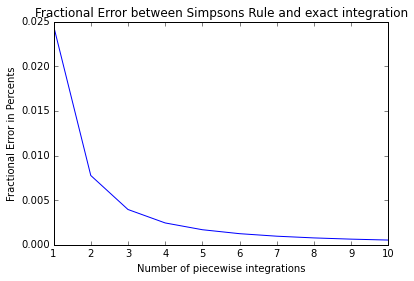
\includegraphics[scale=0.5]{q3.png}
\end{figure}

In the previous question, I wrote functions to compare the accuracy of the
Simpson's Rule of integration and of true integration. Initially, it gave very
accurate results within 0.025 percent of the true value. However, for further 
accuracy, I wrote a function to split Simpson's rule into a number of piecewise
integrations. I then plot the results in Figure \ref{myplot} . 

\end{document}
